\documentclass[a4paper, 12pt]{article}

\usepackage{amsmath}
\usepackage{amssymb}
\usepackage{parskip}
\usepackage{fullpage}
\usepackage{hyperref}
\usepackage{graphicx}
\usepackage{xcolor}
\usepackage{tcolorbox}
\usepackage{changepage}
\usepackage{framed}
\usepackage{biblatex}
\usepackage{filecontents}
\usepackage[italian]{babel}

\usepackage{eso-pic}
\newcommand\BackgroundPic{
    \put(0,0){
        \parbox[b][\paperheight]{\paperwidth}{
            \vfill
            \centering
            
\includegraphics[width=\paperwidth,height=\paperheight]{background}
            \vfill
        }
    }
}

\hypersetup{
    colorlinks=true,
    linkcolor=black,
    urlcolor=blue,
    pdftitle={Laovor PDI},
    pdfpagemode=FullScreen,
}

\begin{filecontents}{references.bib}
@article{penguins,
    author = {Russell, Douglas and Sladen, William and Ainley, David},
    year = {2012},
    month = {10},
    pages = {},
    title = {Dr. George Murray Levick (1876-1956): Unpublished notes on the sexual habits of the Adélie penguin},
    volume = {48},
    journal = {Polar Record},
    doi = {10.1017/S0032247412000216}
}
@article{rowlands2012oxford,
  title={The Oxford Handbook of Animal Ethics},
  author={Rowlands, Mark and Beauchamp, Tom L and Frey, Raymond G},
  year={2012},
  publisher={Oxford University Press}
}
@book{andrews2018routledge,
  title={The Routledge handbook of philosophy of animal minds},
  author={Andrews, Kristin and Beck, Jacob},
  year={2018},
  publisher={Routledge London, New York}
}
@book{rowlands2015can,
  title={Can animals be moral?},
  author={Rowlands, Mark},
  year={2015},
  publisher={Oxford University Press}
}
\end{filecontents}

\addbibresource{references.bib}

\graphicspath{ {./images/} }

\title{
    \textsc{Il ruolo dello Stato democratico nella società umana}
    \\
    {\small \textsc{La democrazia nel sistema giudiziario}}
}

\author{
    \textsc{Paolo Bettelini}
    \\
    \textsc{\large Scuola d'Arti e Mestieri di Trevano (SAMT)}
}

\date{\textsc{\today}}

\linespread{1.25}

\begin{document}

\AddToShipoutPicture*{\BackgroundPic}

\makeatletter
\renewcommand{\maketitle}{
    \vspace*{20pt}
    \begin{adjustwidth}{}{-1in}
        \begin{flushright}
            \begin{tcolorbox}[sharp corners,
                colback=white,
                colframe=white,
                text width=\dimexpr9cm+1in]
                
                \centering
                
                {\LARGE\@title}
                
                \vspace{30pt}
                
                {\large\@author}
                
                \@date
                
                \vspace{20pt}
            \end{tcolorbox}
        \end{flushright}
    \end{adjustwidth}

    \vspace{10cm}

    \begin{adjustwidth}{-1in}{}
        \begin{flushleft}
            \begin{tcolorbox}[sharp corners,
                colback=white,
                colframe=white,
                text width=\dimexpr5cm+1in]
                
                Progetto Didattico Interdisciplinare
                
                Classe I4AC 2022/2023 | PDI
                
                Monica Delucchi, Ursula Holliger
            \end{tcolorbox}
        \end{flushleft}
    \end{adjustwidth}
}
\makeatother

\maketitle

\pagebreak

\tableofcontents
\pagebreak

\section{Introduzione}

\subsection{Il progetto didattico interdisciplinare}

Il progetto didattico interdisciplinare (PDI) è un lavoro originale e personale
con un tema. Il tema generale è "Il ruolo dello Stato democratico nella società umana".
Ho scelto di affrontare questo tema parlando della moralità del sistema giudiziario,
una parte fondamentale di ogni democazia.

\subsection{Biografia}

Durante la mia vita mi sono ritrovato a sviluppare dei pensieri
spesso in discordia con la maggior parte delle persone.
Mediante delle successioni di pensieri logici, ho scoperto autonomamente concetti
come il \textit{determinismo}, senza aver mai avuto nessun contatto con dei testi di filosofia.
\\
Questo lavoro è una riflessione personale che sviluppa i miei pensieri
personali circa la moralità delle cose. Verranno trattate le implicazioni
che questi concetti hanno sulla democrazia e sul sistema giudiziario.

Il documento tratterà la democrazia semplicemente come il concetto di integrare i cittadini
nel governo di una società. Non verranno discussi i diversi modelli di democrazia o di stato
poiché non strettamente attinenti all'argomento.

Le prime sezioni del documento introducono quelli che sono i concetti fondamentali per
sviluppare il mio ragionamento. In seguito verranno trattate
le implicazioni di questi concetti sulla moralità di uno stato e come si potrebbero
ipoteticamente risolvere.

\subsection{Il mio pensiero}

Il mio pensiero consiste in una riflessione circa la moralità delle pene.
Date una serie di affermazioni sulla natura dell'universo, ritengo che l'essere umano
non possegga il libero arbitrio. Questa assenza priva di significato alcuni concetti come la
\textit{pena} o il \textit{merito}. Sostanzialmente, ritengo che sia immorale punire gli esseri
umani per le loro azioni. Ciò non implica che un criminale non debba essere allontanato dalla società,
in quanto un pericolo un provvedimento va comunque effettuato. Tuttavia,
il fatto stesso di punire una persona è intrinsicamente immorale per via
della sua impossibilità di non commettere le azioni che ha commesso.

\pagebreak

\section{Etica e Morale}

\subsection{Definizione}

\paragraph{Morale}
la morale è un insieme di pensieri, decisioni e comportamenti che secondo l'individuo
che li esercita sono \textit{corretti} nei confronti di sé stesso o di terze parti.

\paragraph{Etica}
L'etica è un insieme di pratiche, comportamenti e di norme che vengono applicati
per rispecchiare un'ideologia morale collettiva.

\subsection{Il regno animale}

Seppur molti animali mostrino comportamenti empatici e molte emozioni umani,
molte specie commettono azioni che potrebbero essere giudicate come spregevoli da noi umani.
Senza considerare il bisogno naturale del cacciatore di uccidere, talvolta in maniera brutale,
la preda per sopprivvivere, le azioni considerate da noi immorali riguardando
anche l'ambito sociale fra gli animali e quello sessuali.
Per esempio, alcune specie di pinguini sono stati osservati praticare
pedofilia, necrofilia, stupro e addirittura stupro di altri pinguini soccombenti
\cite{penguins}.

Gli animali dimostrano comunque comportamenti guidati da principi morali
\cite{rowlands2012oxford} \cite{rowlands2015can} \cite{andrews2018routledge}.

\section{Il libero arbitrio}

Il libro arbitrio è un concetto per il quale gli esseri umani
(o, in alcune eccezioni, ogni essere cosciente) sono in grado di decidere e agire secondo la propria volontà.
L'essere è quindi libero di arbitrare le proprie azioni secondo la sua volontà.

 \section{Il determinismo}

\subsection{Definizione}

Il determinismo è una corrente di pensiero che esprime l'idea
che gli eventi dell'universo siano completamente determinati e prevedibili.
\\
Vi sono diverse versioni di questo pensiero e
molti filosofi hanno sviluppato i concetti, fra cui Platone, Kant,
Nietzsche e Confucio.

\subsubsection{Determinismo duro}

Il determinismo duro è la versione più severa del determinismo.
Questo pensiero indica che tutti gli eventi siano strettamente
determinabili dagli eventi dell'universo precedenti.
Conoscendo l'esatto stato dell'universo in un dato istante \(t_n\), è possibile
determinare un qualsiasi istante futuro \(t_{m > n}\).

Questo ideologia è in contrapposizione con il libero arbitrio.
Dal momento che tutti gli eventi nell'universo sono determinati da altri fattori determinati
o detemrinabili, i processi biologici che ci permettono di prendere delle decisioni e di pensare
sono soggette al determinismo duro, in quanto facenti parti di un sistema fisico esistente nell'universo.

\subsubsection{Compatibilismo}

Il compatibilismo è una corrente di pensiero che prevede una compatibilità
fra il libero arbitrio ed il determinismo. Un'accezione generica di questa ideologia
implica che l'uomo abbia infatti il potere di scegliere liberamente secondo la sua volontà.

\subsection{Determinismo nella fisica}

Il mondo in cui viviamo è governato dalla meccanica.
Tutte le nostre azioni quotidiane sono governate dalla meccanica.
Guidare l'auto, fare cadere un oggetto, camminare etc. sono tutte azioni
che rispettano delle leggi fisiche ben conosciute. \\
Agli inizi del XX secolo la comunità scientifica ha cominciato ad esplorare ciò che
è la meccanica quantistica. Queste nuovi leggi secondo le quali il nostro universo funziona
ad un livello microscopico, hanno generato diverse critiche verso il determinismo.
Queste leggi potrebbero infatti indicare che l'universo non si basa unicamente su eventi deterministici ma anche eventi casuali.

\subsubsection{Principio di indeterminazione di Heisenberg}

Il principio di indeterminazione di Heisenberg è molto importante nelle discussioni
legale al determinismo e alla natura intrinseca dell'universo.
Questo concetto indica infatti che, considerando un oggetto quantistico (di dimensioni molto piccole),
l'ammontare di conoscenza sulla sua velocità è inversamente proporzionale all'ammontare
di conoscenza sulla sua posizione.
Se conosciamo esattamente la posizione di un oggetto, non sappiamo nulla sulla sua velocità.
Se conosciamo esattamente la sua velocità, non sappiamo nulla sulla posizione. Se siamo un po'
incerti sulla sua velocità, siamo anche un po' incerti sulla sua posizione.
La nostra conoscenza \textit{simultanea} di alcune proprietà è vincolata da delle leggi fisiche. \\
Questa affermazione può sembrare assurda e priva di senso, ma nel campo quantistico
alcune proprietà sono descritte da delle probabilità piuttosto che da dei valori sempre concreti.

Considerando questo fenomeno fisico possiamo giungere ad una contraddizione nel determinismo.
Non è possibile conoscere lo stato dell'universo ad un certo istante se non possiamo
conoscere simultaneamente tutte le proprietà del nostro sistema.

\subsubsection{Eventi casuali}

La fisica quantistica è governata da funzioni probabilistiche.
Una funzione probabilistica è una funzione che descrive un fenomeno. Essa
esprime la possibilità che ogni possibile risultato avvenga. Per esempio,
una funzione probabilistica potrebbe descrivere l'altezza delle persone.
Scegliendo una persona qualsiasi in una piazza, abbiamo un'alta probabilità che la sua altezza
sia all'incirca 170cm, mentre abbiamo una probabilità più bassa che la persona sia alta 150cm oppure 190cm.
Questo è ciò che descrive una funzione di questo tipo, notiamo come ogni persona abbia il 100\% di probabilità
di avere un'altezza (la funzione descrive tutti i possibili risultati).
Per quel che concerne la meccanica quantistica basti pensare alla posizione di un elettrone. La posizione di un elettrone
di un sistema può essere descritta da una \textit{funzione d'onda}. Questa funzione descrive
la probabilità di misurare l'elettrone in un certo punto. Per esempio, considerando un elettrone libero
di trovarsi su una linea, potrebbe essere molto probabile che esso venga misurato essere nello spazio centrale, mentre
poco probabile che si trovi agli estremi.

\begin{figure}[h]
    \centering
    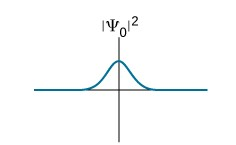
\includegraphics[width=0.5\textwidth]{wavefunction.jpg}
    \caption{Funzione d'onda}
\end{figure}

La natura deterministica dell'universo è dunque strettamente legata all'esistenza di
eventi puramente casuali.

\paragraph{Un evento pseudo-casuale} o un numero pseudo-casuale è un evento
che approssima una probabilità ma sono è realtà deterministico.
Il lancio di un dado o di una moneta sono degli eventi pseudo-casuali.
La probabilità che una moneta atterri in una certa maniera è 50\%, tuttavia,
questo risultato è ben definito dalle leggi fisiche della meccanica. \\
Un altro esempio sono i numeri randomici generati dai computer, essi sono infatti
pseudo-casuali. Il computer sfrutta il numero di millisecondi passati dall'1 gennaio 1970 (unix-time).
Questo valore è molto volatile e per cui ottimale per generare una distribuzione
omogenea di numeri casuali. \\
Ci sono molti valori volatili in natura. Misurare la temperatura con un termometro
e considerare alcune cifre dalla decima cifra in poi dopo la virgola risulta
in un numero quasi casuali.
Tutti questi fenomeni possono essere ricostruiti date le condizioni di partenza.

\paragraph{Un evento puramente casuale} è un qualsiasi evento che potrebbe svolgersi in maniera differente se l'universo venisse riavvolto per ripetere nuovamente tale evento, senza che l'esecuzione dell'evento a priori abbia alcun effetto sulla nuova esecuzione.

Se nell'universo sono presenti eventi puramente casuali il determinismo non è corretto
in quanto non tutti gli avvenimento sono deducibili dagli eventi precedenti.

Gli eventi casuali presenti nella meccanica quantistica sono puramente casuali
oppure possono essere deducibili da altri fattori (pseudo-casuali)?
Questa è la domanda saliente circa il determinismo.
Se gli eventi puramente casuali dovessero esistere l'universo non si potrebbe basare unicamente
su regole deterministiche.
La scienza non è mai riuscita a dimostrare o sfatare nessuna delle due ipotesi.

\subsection{Determinismo nell'anatomia}

La seguente sezione tratta in maniera generale il funzionamento del cervello
e come prendiamo ogni decisione.

Il cervello è una macchina molto complessa che nessuno
comprende pienamente. Tuttavia, la scienza riesce a spiegare a grandi linee
il sistema decisionale. Questo sistema si basa su tante piccole strutture cellulari
facenti parti del sistema neuroso, i \textit{neuroni}.

\begin{figure}[h]
    \centering
    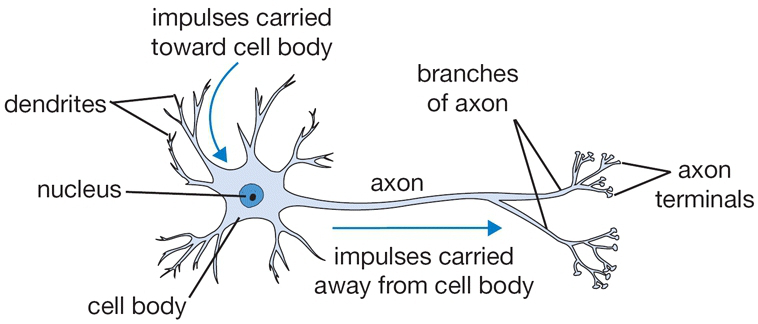
\includegraphics[width=0.75\textwidth]{neuron.png}
    \caption{Struttura neuronale}
\end{figure}

[...]

Possiamo dunque dedurre che ogni decisione mai presa da ognuno di noi è
sostanzialmente dipendente da 3 fattori:
\begin{enumerate}
    \item Configurazione genetica iniziale
    \item Eventi vissuti
    \item Ambiente circostante
\end{enumerate}

\paragraph{Configurazione genetica iniziale}
Il modo di pensare è certamente diverso fra persona e persona.
Uno dei fattori molto importanti è la configurazione anatomica iniziale del cervello,
ossia la configurazione iniziale di sinapsi, neuroni etc. alla nascita.

\paragraph{Eventi vissuti}
Ogni evento vissuto può modificare la nostra capacità di pensare.
Un evento può consistere in un'interazione fisica o semplicemente qualcosa di visto.
Durante la vita le configurazioni delle sinapsi evolve costantemente. Provare certe esperienze
o trovarsi in certe situazioni può certamente alterare la nostra capacità cognitiva.
Un evento può per esempio consistere nell'alterazione fisica del cervello, come per esempio
un intervento di leucotomia oppure la malattia del morbo di Alzheimer.

\paragraph{Ambiente circostante}
Al momento di prendere una decisione l'ambiente circostante è uno dei principali fattori
principali. A seconda della situazioni, cerchiamo di prendere una decisione auspicabile
per affrontare quest'ultima.

\subsection{Determinismo nella filosofia}

\subsection{Determinismo nella politica}

\subsection{Implicazioni nella moralità}

Assumendo il determinismo si giunge ad un concetto che può essere molto pericoloso per una società
e le persone stesse. Questo concetto è la perdita del significato della colpa o della responsabilità, del merito e altri simili.

\section{Il sistema giudiziario}

\subsection{Definizione e democrazia}

Il sistema giudiziario che si occupa di condannare gli atti illeciti
al fine di mantenere il quieto vivere.

\subsection{Funzionamento}

\subsection{Nella storia}

\subsubsection{La legge del taglione}


\subsubsection{La legge del contrappasso}
\subsubsection{La ghigliottina}
\subsubsection{Cesare Beccaria}

Cesare Beccaria (1738-1794) è stato un giurista e filosofo francese.
Nel 1764 pubblica "Dei delitti e delle pene" (cita) 
dove esamna una serie di difetti nel sistema dell'epoca che imponevano una giustizia equa.
Questa'opera è molto importante poiché delimita il peccatto (peccato religioso
che viene giudicato da Dio) da ciò che bisogna considerare da un punto di vista giuridico,
applicando leggi eque e uguali per tutti.

Cesare Beccaria era contrario alla pena di morte e alla tortura, infatti,
voleva dimostrare che queste metodologie fossero inefficaci e disumani.
Una delle sue idee primarie era l'importanza di prevenire un delitto piuttosto che punirlo.

\subsection{Moralità nel sistema giudiziario}

[punto principale del PDI] \\
Dati i ragionamenti logici nelle sezioni precedenti, è morale punire
un criminale?

\subsection{Implementazione alternativa}

\section{Conclusione}

\pagebreak

\listoffigures

\pagebreak

%\nocite{*} % cite all entries

\printbibliography[heading=subbibliography]

\end{document}